\documentclass[tikz,border=2pt]{standalone}
\usepackage{amsmath}
\usetikzlibrary{arrows.meta}
\begin{document}
% (T,S) cost recursion for T = 2, S = 2, lead time 1, demand D in {0,1,2} w.p. 1/4, 1/2, 1/4,
% h = 1, b = 4, K = 6: L(2) = 1, L(1) = 5/4, L(0) = 4, V(1,x) = L(x) + K, V(2,2) = 1 + E[V(1,2-D)] = 71/8.
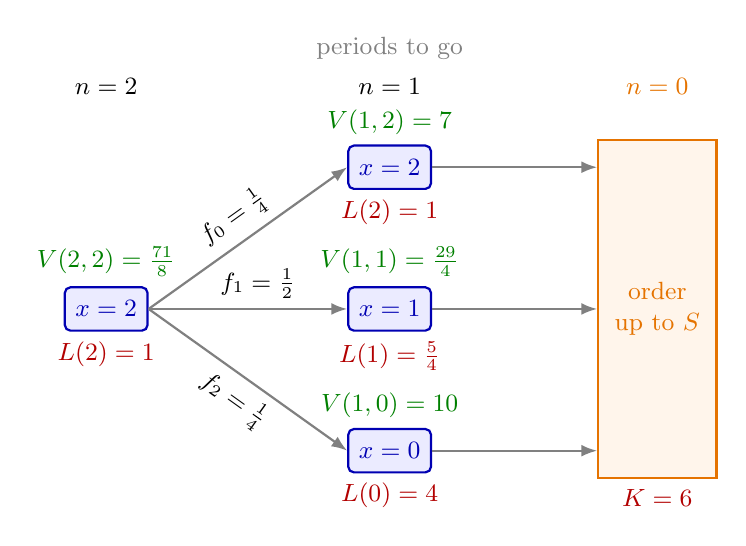
\begin{tikzpicture}[font=\small, >={Latex[length=2mm]},
  st/.style={draw=blue!70!black, thick, rounded corners=2pt, fill=blue!8, minimum width=1.05cm, minimum height=0.55cm, text=blue!70!black}]
  % column headers
  \node[anchor=south] at (0,4.4) {$n=2$};
  \node[anchor=south] at (3.6,4.4) {$n=1$};
  \node[anchor=south, orange!90!black] at (7.0,4.4) {$n=0$};
  \node[anchor=south, gray] at (3.6,4.85) {periods to go};
  % states
  \node[st] (r) at (0,1.8) {$x=2$};
  \node[st] (a) at (3.6,3.6) {$x=2$};
  \node[st] (b) at (3.6,1.8) {$x=1$};
  \node[st] (c) at (3.6,0.0) {$x=0$};
  % hitting set n = 0
  \node[draw=orange!90!black, thick, fill=orange!8, minimum width=1.5cm, minimum height=4.3cm, align=center] (k) at (7.0,1.8) {};
  \node[orange!90!black, align=center] at (7.0,1.8) {order\\up to $S$};
  % transitions with demand probabilities
  \draw[->, thick, gray] (r.east) -- (a.west) node[pos=0.5, above, sloped, black] {$f_0=\tfrac{1}{4}$};
  \draw[->, thick, gray] (r.east) -- (b.west) node[pos=0.55, above, black] {$f_1=\tfrac{1}{2}$};
  \draw[->, thick, gray] (r.east) -- (c.west) node[pos=0.5, below, sloped, black] {$f_2=\tfrac{1}{4}$};
  \foreach \s in {a,b,c} {\draw[->, thick, gray] (\s.east) -- (\s.east -| k.west);}
  % running costs (red) and values (green)
  \node[red!70!black, anchor=north] at (r.south) {$L(2)=1$};
  \node[red!70!black, anchor=north] at (a.south) {$L(2)=1$};
  \node[red!70!black, anchor=north] at (b.south) {$L(1)=\tfrac{5}{4}$};
  \node[red!70!black, anchor=north] at (c.south) {$L(0)=4$};
  \node[green!50!black, anchor=south] at (r.north) {$V(2,2)=\tfrac{71}{8}$};
  \node[green!50!black, anchor=south] at (a.north) {$V(1,2)=7$};
  \node[green!50!black, anchor=south] at (b.north) {$V(1,1)=\tfrac{29}{4}$};
  \node[green!50!black, anchor=south] at (c.north) {$V(1,0)=10$};
  \node[red!70!black, anchor=north] at (k.south) {$K=6$};
\end{tikzpicture}
\end{document}
